% ==============================
\section{lezione del 19-03-26}
Nella scorsa lezione abbiamo visto come calcolare la probabilità che un evento A 
si verifichi k volte in un ordine qualsiasi
\[
    P(E) = \frac{N!}{k!(N - k)!}p^k(1 - p)^{N - k} = \binom{N}{k}p^k(1 - p)^{N - k}
\]
conouscita anche come \textit{formual di Bernoulli}

Proviamo a vedere un un esercizio: 
\begin{itemize}
    \item In un urna sono contenute $M$ biglie, ve ne sono $b$ bianche e $M - b$ di diveso colore.
    \item Si estrae 5  volte una biglia, rimettendola nell'urna prima dell'estrazione successiva.
    \item Quale è la probabiltà $P$ di ottenere nelle 5 estrazioni, 3 volte una biglia bianca.
        e 2 volte una biglia di diverso colore
\end{itemize}
Notiamo che la probabilità di estratte una biglia bianca è
\[
    p = \frac{b}{M}
\]
dove $p$ è la probabiltà di successo della singla prova.
possiamo quindi applicare la formula di Bernoulli e otteniamo
\[
    \binom{N}{k}p^k(1 - p)^{N-k} = \binom{5}{3}\left ( \frac{b}{M} \right)^3\left ( 1 -\frac{b}{M}\right)^2
\]
\subsection{Esperimenti non indipendenti}\label{sub:Esperimenti non indipendenti} % (fold)
Nella pratica si verificano spesso esperimenti \textbf{non indipendenti}. In questa
classe ricadono i casi nei quali il primo esperimento modificana lo spazione campione 
$\Omega_2$ del secondo. \\ 

Concetriamoci su un esempio anche questa volta
\begin{importantbox}
    \textit{Si calcoli la probabilità che estraendo due carte da un mazzo di 40, entrambe
    risultino di fiori. Si assuma che il mazzo di carte non sia truccato.}
\end{importantbox}
Guardiamo alle probabiltà dei singoli eventi 
\begin{itemize}
    \item $A$ = \{Nella prima estrazione si estrae una carta di fiori\}
    \item $B$ = \{Nella seconda estrazione si estrae una carta di fiori\}
    \item $B|A$ = \{Nella seconda estrazione si ottiene una carta di fiori dopo che nella prima
si è ottenuta una carta di fiori\}
\end{itemize}
\begin{itemize}
    \item  Si può descrivere questo esperimento come composto da due
esperimenti singoli costituiti dall’estrazione di una singola carta dal mazzo, otteniamo: 
    \[
        P(A) = \frac{1}{4}, \quad P(B|A) = \frac{9}{39}
    \]
    \[
        P(A \cap B) = P(B|A)P(A) =\frac{9}{39}\cdot\frac{10}{40} = \frac{3}{52}
    \]
    Adesso per calcolari la probabiltà dell'evento $B$ utilizziamo il \textit{teorema della probabiltà totale}
    \[
        P(B) = P(B|A)P(A) = P(B|\overline A)P(\overline A) = \frac{1}{4}
    \]
    Notiamo che $P(A) = P(B)$, risulta quindi che in media la probabilità di estrarre 
    una carta di fiori al secondo lancio non varia rispetto alla prima.
\item Un altro approccio consiste nel notare che il  numero di possibili risultati è dato dal numero di combinazioni di 40
oggetti presi 2 a 2:
\[
    C_{40,2} = \binom{40}{2} = \frac{40!}{2!\cdot38!}
\]
e che il numero di risultati favorevoli è dato dal numero di possibili modi in
cui si possono disporre 10 oggetti (le carte a fiori) a coppie; tale
numero è dato dalle combinazioni di 10 oggetti presi 2 a 2:
\[
    C_{10, 2} = \binom{10}{2} = \frac{10!}{2!\cdot8!}
\]
Otteniamo quidi che la probabilità $P$ di estrare due carte a fiori è
\[
    P = \frac{\binom{10}{2}}{\binom{40}{2}} = \frac{3}{52}
\]
\end{itemize}
% subsection Esperimenti non indipendenti (end)
\subsubsection{Canale di comunicazione binario simmetrico}\label{sub:Canale di comunicazione binario simmetrico} % (fold)
Consideriamo di avere un sistema di comunicazione dove: 
\begin{itemize}
    \item 1 è trasmesso con probabiltà $p = 0.3$ e 0 con $(1 - p) = 0.7$
    \item La probabiltà di errore è $p_e$ (indipendente dal simbolo trasmesso)
    \item Defiano $T_0 = $ \{è stato \textit{trasmesso} 0 \} e $T_1 = $ \{è stato \textit{trasmesso} 1 \}
    \item Defiano $R_0 = $ \{è stato \textit{trasmesso} 0 \} e $T_1 = $ \{è stato \textit{trasmesso} 1 \}
\end{itemize}
Vogliamo calcolare $P[T_0|R_0]$ ossia la probailità che una volta trasmesso 
uno zero venga effettivamente ricevuto.
% subsection Canale di comunicazione binario simmetrico (end)
\begin{center}
    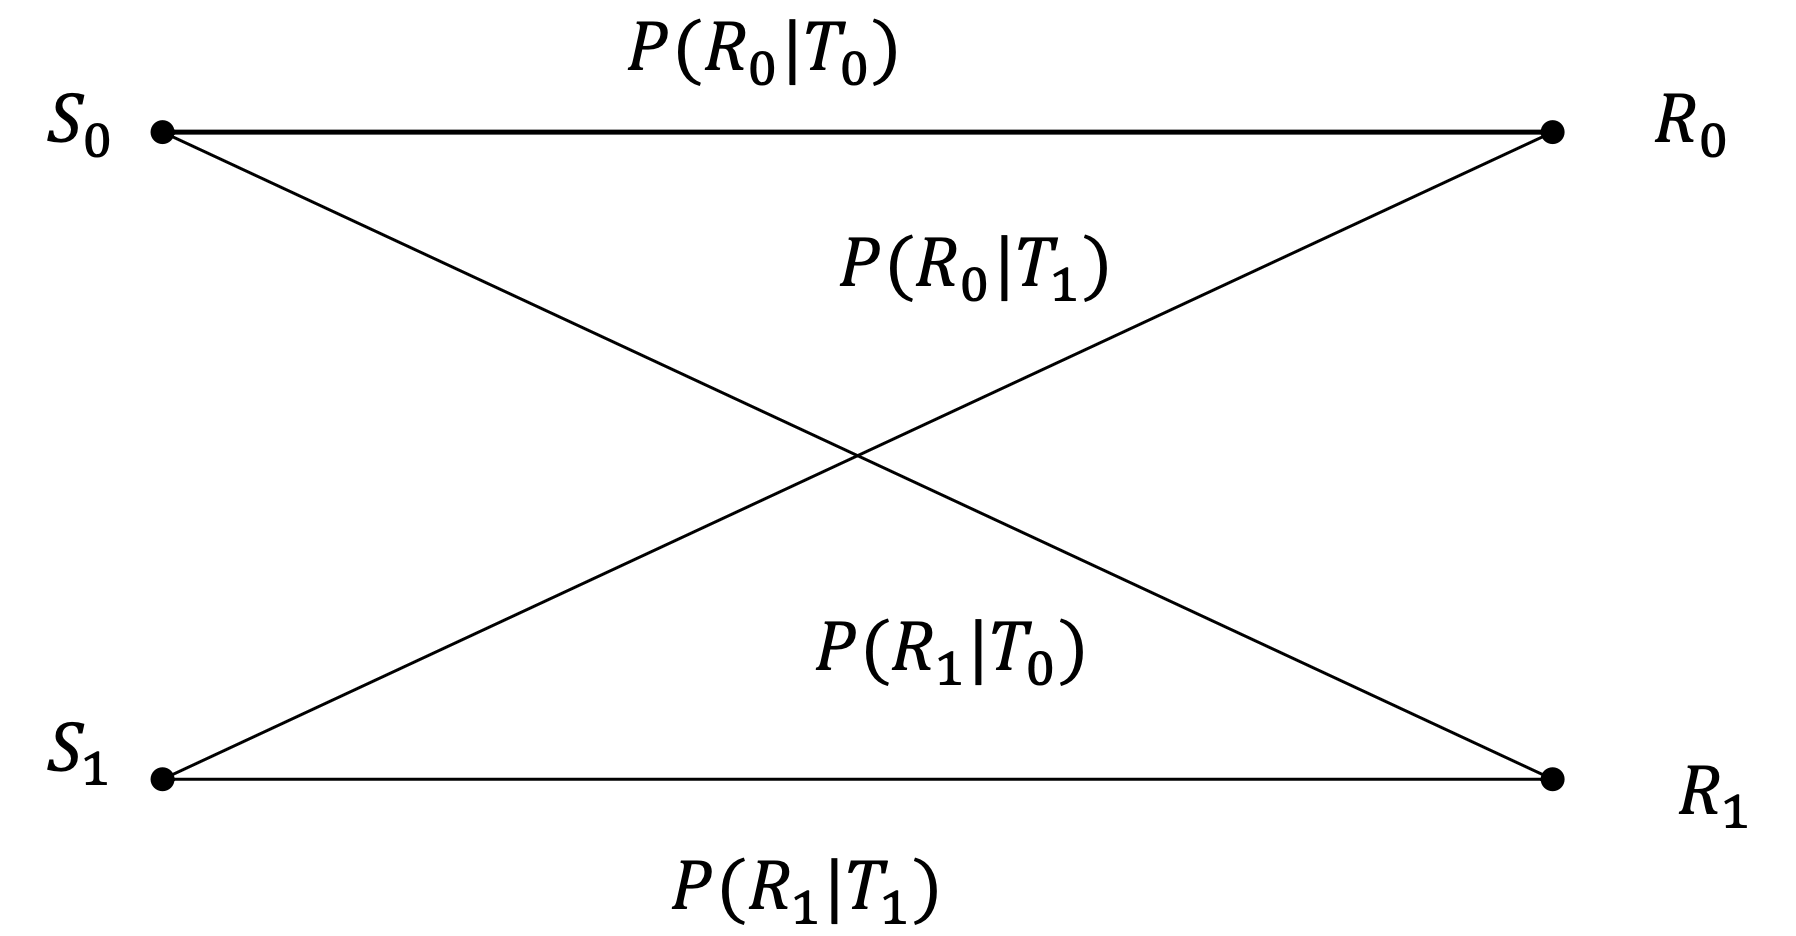
\includegraphics[scale=0.35]{../images/prob_cond_canale_comunicazione.png} 
\end{center}
Analizziano due casistiche:

\begin{itemize}
    \item $p_e = 0$ in questo caso otteniamo 
        %  da fare (foto lavagna sul teleefono)
\end{itemize}


\subsection{Variabili aleatorie}\label{sub:Variabili aleatorie} % (fold)
Una \textit{variabile aleatoria}(o casuale) è una funzione che associa un numero reale  
a ogni possibile esito di un esperimento casuale, mappando lo spazio campionario $\Omega$
nell'insieme dei numeri reali $\mathbb R$. Essa trasforma eventi non numerici in dati 
quantitativi, permettendo l'analisi probabilistica.
% subsection Variabili aleatorie (end)
\begin{center}
    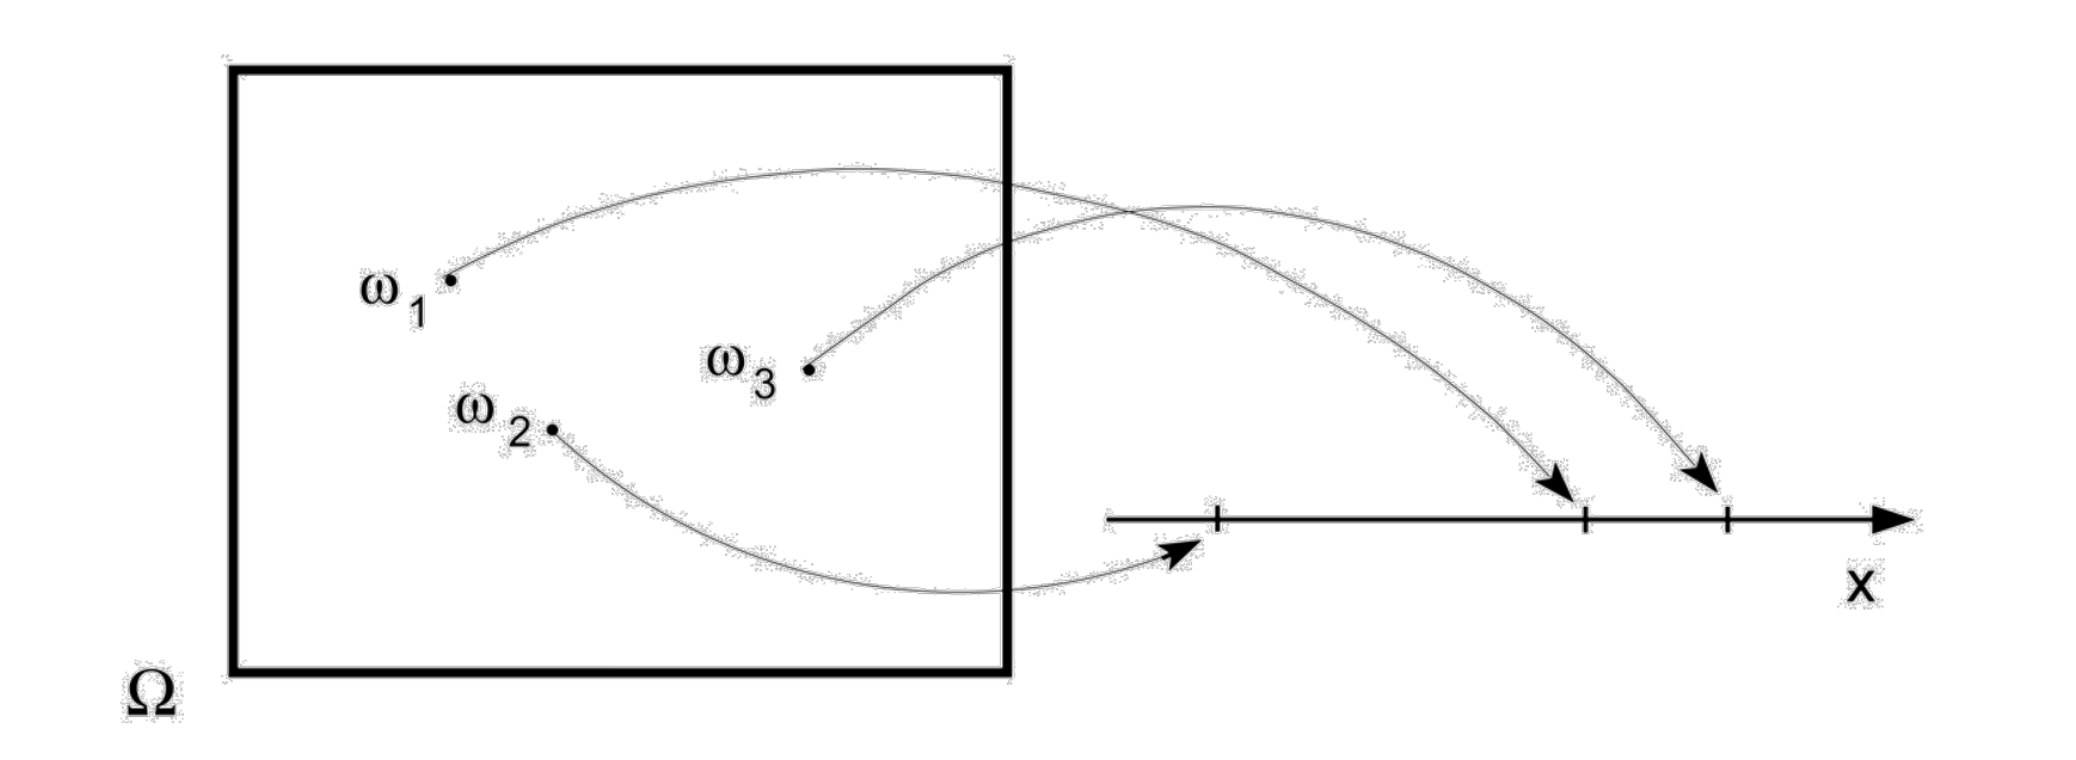
\includegraphics[scale=0.35]{../images/variabili_aleatorie.png} 
\end{center}
Tutti i sottoinsiemi di $\mathbb R$ che si ottengono come unione o intersezione
di sottoinsiemi del tipo $\{X(\omega) \leq a\}$ sono ancora degli eventi quindi
è possible assegnagli una probabilità 
\[
    \{ b \leq X(\omega) \leq  a\} = \{X(\omega) \leq a \} - \{X(\omega) \leq b \}, \quad b \geq a
\]
\textbf{Nota:} in seguito le variabile aleatorie saranno rappresentato da letter maiuscole
omettendo la dipendenza da $\omega$, quindi avremmo $Y$ invece di $Y(\omega)$ 
\subsubsection{Funzione di distribuzione}\label{sec:Funzione di distribuzione} % (fold)
\begin{importantbox}
   Si indica \textbf{funzione di distribuzione} di probabilità di una variabile 
   aleatoria $X$, la funzione: 
   \[
       F_X(x) \triangleq P(\{X \leq  x\})
   \]
\end{importantbox}
La definizione di variabile aleatore ci assicura che $F_X(x)$ esiste $\forall x \in \mathbb R$. 
Notiamo anche che il simbolo $x$ indica un valore generico ma fissato che identifica
l'event $\{X \leq x\}$.
% subsubsection Funzione di distribuzione (end)
\subsubsection{Proprità della funzione di distribuzione}\label{sec:Proprità della funzione di distribuzione} % (fold)
\begin{enumerate}
    \item $ 0 \leq F_X(x) \leq 1$
    \item $\lim_{x \to -\infty} F_X(x) = F_X(-\infty) = p(\{X \leq -\infty\}) = 0 $
    \item $\lim_{x \to +\infty} F_X(x) = F_X(+\infty) = p(\{X \leq +\infty\}) = 1 $
    \item $\forall x_1,x_2 \in \mathbb R \mid x_1 < x_2 \implies F_X(x_1) \leq F_X(x_2)$ 
    \item $P(x_1 < X \leq x_2) = F_X(x_1) - F_X(x_2)$ 
    \item La funzione di distribuzione è \textbf{continua da destra}. Quindi nei punti di
    discontinuità il valore della funzione coincide con il suo limite destro: 
    \[
        F_X(x^+) = \lim_{h \to 0^+}F_X(x + h) = F_X(x)
    \]
    \item Se la funzione di distribuzione presenta una discontinuità di prima
    specie nel punto $x = \overline x$, la differenza tra il suo limite destro e sinistro
    è pari alla probabilità dell’evento $\{X = \overline x\}$
    \[
        P(\{X = \overline x\}) = F_X(\overline x^+) - F_X(\overline x^-)
    \]
\end{enumerate}
Date queste proprietà e possibile determinare la probabilità di di qualunque evento
$\{X \in I\}$ essento $I$ un insieme reale di somma di intervalli aperti, chiusi, semiaperti
dell'asse reale. La conoscenza di $F_X(\cdot)$ rappresenta la \textbf{descrizione statisica completa}
della variabile aleatoria $X$.
\begin{importantbox}
   Una descrizione statistica equivalente, ma a volte più semplice, è
    data dalla funzione massa di probabilità, nel caso di v.a. discrete, e
    dalla funzione densità di probabilità, nel caso di v.a. continue 
\end{importantbox}
% subsubsection Proprità della funzione di distribuzione (end)

\subsection{Variabili aleatori discrete}\label{sub:Variabili aleatori discrete} % (fold)
\begin{importantbox}
    Una v.a. si dice discreta se assume un numero finito
    o una infinità numerabile di valori distinti: $x_1, x_2, \dots ,x_i, \dots$ 
    \[
        \textbf{Funzione massa di probabilità}: p_X(x) = P(\{X = x\}) 
    \]
    È diversa da zero solo nei punti $x = x_1, x_2, \dots$
\end{importantbox}
Dato che gli eventi $\{X = x_i\}$ sono una partizione i $\Omega$ possiamo dire che 
\[
    \sum_i p_X(x_i) = \sum_i P(\{X = x_i\}) = 1
\]
Adesso diamo una definizione della massa di probabiltà come limite della frequenza
relativa
\[
    p_X(x_i) = P(\{X = x_i\}) = \lim_{N \to +\infty} \frac{n(x_i)}{N}
\]
questa definizione implica che:
\begin{itemize}
    \item L'esperimento va ripetuto $N$ volte
    \item Per ogni $x_i$ va  calcolato il numero di volte $n(x_i)$ in cui tale valore si è presentato
    \item Per ogni $x_i$ calcolare la frequnza di presentazione:
        \[
            \hat p(x_i) = \frac{n(x_i)}{N}
        \]
\end{itemize}
Aggiungiamo anche che se abbiamo una variabile aleatoria che:
\begin{itemize}
    \item Assume valore 1 con probabiltà $p$
    \item Assume valore 0 con probabiltà $1 - p$
\end{itemize}
sono dette \textbf{varbili aleatore di Bernoulli}. Si scrive anche $X \in \textit{Bernoulli}(p)$
% subsection Variabili aleatori discrete (end)